% !TeX spellcheck = pt_BR
\documentclass[tese_patricia]{subfiles}
\begin{document}


\begin{comment}
	\nomenclature[F,01]{$\Omega$}{Domínio computacional;}
	\nomenclature[F,02]{$\globalModel$}{Domínio computacional global;}
	\nomenclature[F,03]{$\localModel$}{Domínio computacional local;}
	\nomenclature[F,04]{$\overlappingZone$}{Zona de superposição;}
	\nomenclature[F,05]{$\gluingZone$}{Zona de colagem;}
	\nomenclature[F,06]{$\freeZone$}{Zona livre;}
	\nomenclature[F,07]{$\lagrangeMultiplier$}{Campo de multiplicadores de Lagrange;}
	\nomenclature[F,08]{$k_{0},k_{1}$}{Constantes dos operadores de acoplamento;}
	\nomenclature[F,09]{$L^{2}$}{Operador de acoplamento de ordem 0;}
	\nomenclature[F,10]{$H^{1}$}{Operador de acoplamento de ordem 1;}
	\nomenclature[F,11]{$\arlequinWF$}{Função ponderadora;}
	\nomenclature[F,12]{$k_{a}$}{Constante arbitrária do método de Arlequin;}
	\nomenclature[F,13]{$\lagSolution$}{Espaço vetorial das funções aproximadoras do campo de multiplicadores de Lagrange;}
	\nomenclature[F,14]{$\lagTest$}{Espaço vetorial das funções ponderadoras do campo de multiplicadores de Lagrange;}
	\nomenclature[F,15]{$\lagrangeMultiplierWFh$}{Função ponderadora pertencente ao espaço $\lagTest$;}
	\nomenclature[F,16]{$\chi$}{Função lógica para determinação do pertencimento de um ponto à $\gluingZone$;}
	\nomenclature[F,17]{$\tauArlequin$}{Parâmetro de estabilização da técnica RBSAM;}
	\nomenclature[F,18]{$\mathbf{R}_{L}$}{Resíduo da versão semidoscreta da equação de restrição}
	\nomenclature[F,19]{$\LagrangeMultiplier$}{Vetor nodal dos graus de liberdade respectivo aos multiplicadores de Lagrange}
	\nomenclature[F,20]{$\tau_{A},\tau_{A}^{0},\tau_{A}^{1}}{Parâmetros auxiliares para a determinação de $\tauArlequin$;}
	\nomenclature[F,21]{$\tau_{B},\tau_{B}^{0},\tau_{B}^{1}}{Parâmetros auxiliares para a determinação de $\tauArlequin$;}
	\nomenclature[F,22]{$\tau_{C},\tau_{C}^{0},\tau_{C}^{1}}{Parâmetros auxiliares para a determinação de $\tauArlequin$;}
	\nomenclature[F,23]{$\tau_{D},\tau_{D}^{0},\tau_{D}^{1}}{Parâmetros auxiliares para a determinação de $\tauArlequin$;}
	\nomenclature[F,24]{$\tau_{E},\tau_{E}^{0},\tau_{E}^{1}}{Parâmetros auxiliares para a determinação de $\tauArlequin$;}
	\nomenclature[F,25]{$\tau_{E},\tau_{E}^{0},\tau_{E}^{1}}{Parâmetros auxiliares para a determinação de $\tauArlequin$;}	
	\nomenclature[F,26]{$\mathbf{M_{\lambda}},\mathbf{t}, \mathbf{j}, \mathbf{k}, \mathbf{p}, \mathbf{\boundary}$}{Matrizes elementares da formulação usadas na definição de $\tauArlequin$, com base dos termos de acoplamento, convectivos, inerciais, viscosos, pressão e de acoplamento (?) respectivamente;}
	\nomenclature[F,27]{$C$}{Corda: distância entre o bordo ataque e de fuga do aerofólio;}	
	\nomenclature[F,28]{$\theta, \theta_{max}, \theta_{min}$}{Ângulo de ataque; Ângulo de ataque máximo; Ângulo de ataque mínimo;}	
	\nomenclature[F,29]{$f_{f}$}{Frequência de oscilação;}

	
\end{comment}

% ---------------------------------------------------------- 
% Métodos de malhas sobrepostas
% ----------------------------------------------------------
\chapter[Método de Arlequin estabilizado]{Técnica de decomposição de domínios através do Método de Arlequin estabilizado - RBSAM} \label{capitulo:Cap6}
% ----------------------------------------------------------

Com intuito de superar as dificuldades encontrados com a técnica de decomposição de domínios apresentada no Cap. \ref{capitulo:Cap5}, neste capítulo será apresentado o método multiescala Arlequin que permite também levar em conta efeitos localizados através do uso de um modelo local mais refinado superposto a um modelo global com discretização mais grosseira. No método Arlequin, o processo é realizado através do cruzamento e colagem entre os modelos em uma zona de colagem através da utilização de um operador de acoplamento.

A primeira parte deste capítulo será dedicada a descrever o método clássico de Arlequin, introduzido por \citeonline{Dhia:1998}. Na sequência será apresentada  a técnica de estabilização (RBSAM) introduzida por \citeonline{FernandesEtAll:2020} para o método de Arlequin no contexto de escoamentos incompressíveis. Na sucessão do capítulo, a extensão de tal metodologia para problemas de contorno móveis será exibida. E, por fim, exemplos de validação serão avaliados.

\section{Método Arlequin}

O método Arlequin, introduzido por \citeonline{Dhia:1998}, consiste na superposição de um domínio local a um domínio global, em região efeitos localizados. Os modelos, local e global, são acoplados em uma zona de colagem através de um operador de acoplamento conveniente.

O  método de Arlequin, de acordo com \citeonline{DhiaR:2005}, é baseado em três principais ideias (ver Fig. \ref{fig:DomLocalGlobal}):

\begin{itemize}
	\item Um domínio local $\localModel$ é sobreposto em um domínio global  $\globalModel$ em uma zona de interesse de modo a representar efeitos locais;
	\item Os modelos são colados um ao outro em uma subzona da zona de superposição ($\overlappingZone$), chamada de zona de colagem ($\gluingZone$), através de um operador de acoplamento conveninente;
	\item  Garante-se a distribuição da energia entre os modelos através do emprego de uma função ponderadora, definida a partir da partição da unidade;
\end{itemize}

\begin{figure}[htb!]
	\centering 
	%\vspace{-1em} % Diminui o espaço antes da figura
	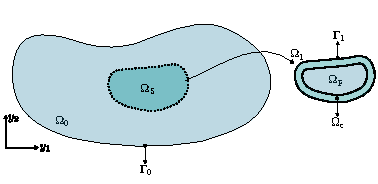
\includegraphics[scale=1.0,trim=0cm 0cm 0cm 0.0cm, clip=true]{Imagens/Cap6/dominioArlequin.pdf}	
	\caption{Domínio local e global.}
	\label{fig:DomLocalGlobal}
	%\vspace{-1em} % Diminui o espaço antes da figura
\end{figure}

Dessa forma, o domínio computacional do problema é definido por:

\begin{align}
	\Omega = \globalModel + \localModel, 
\end{align}

\noindent a zona de superposição, $\overlappingZone$, pode ser definida matematicamente da seguinte forma:

\begin{align}
	\overlappingZone = \globalModel \cap \localModel, \\
	\overlappingZone = \gluingZone \cup \freeZone, \\
	\overlappingZone > 0, 
\end{align}

\noindent sendo  $\freeZone$ a chamada zona livre.

Umas das formas mais comuns de se realizar o acoplamento entre os modelos na zona de colagem $\gluingZone$ é através da aplicação de campos de multiplicadores de Lagrange. Uma forma generalizada de representar os operadores de acoplamento é apresentada em \citeonline{DhiaR:2002}, da maneira que se segue:

\begin{align}
	(\lagrangeMultiplier,\Delta u) =  \int_{\gluingZone} k_{0}[\lagrangeMultiplier \cdot \Delta \mathbf{u} ] + k_{1}[\straintensor (\lagrangeMultiplier) : \straintensor (\Delta \mathbf{u})] \ d\Omega_{c},
\end{align}

\noindent onde $\lagrangeMultiplier$ é o campo de multiplicadores de Lagrange, $\Delta \mathbf{u} = \uglobal |_{\gluingZone} - \ulocal |_{\gluingZone}$ é a diferença entre os campos acoplados na zona de colagem. $k_{0}$ e $k_{1}$ são constantes estritamente positivas. 

Quando $k_{0} > 0$ e $k_{1} = 0 $ têm-se o operador de acoplamento $L^{2}$. Esse acoplador estabelece a continuidade de ordem 0 do campo compatibilizado, que significada que ele garante no sentido de forma fraca, a continuidade das variáveis ao longo da zona de colagem. Para valores $k_{0} > 0$ e $k_{1} > 0 $ obtêm-se o operador de acoplamento $H^{1}$, estabelecendo continuidade de ordem 1 do campo compatibilizado, garantindo no sentido de forma fraca, a continuidade de uma combinação de variáveis e seu Laplaciano \cite{GuidaultAndBelytschko2007}.

O sucesso do método, indiferente do tipo de operador adotado, depende da escolha apropriada dos parâmetros $k_{0}$ e $k_{1}$. Para o acoplamento utilizando $L^{2}$, devido a simplicidade da aplicação da restrição dos campos compatibilizados na zona de colagem, o condicionamento do sistema depende fortemente da adoção do parâmetro $k_{0}$, sendo esta uma das razões pela qual a maioria dos trabalhos realizados utilizando o método Arlequin aplica o operador $H^{1}$. A obtenção de parâmetros ótimos para o método pode ser uma tarefa difícil, sendo esse um dos fatores que levaram \citeonline{FernandesEtAll:2020} ao desenvolvimento da técnica RBSAM que será discutida na próxima seção.

A definição do espaço de funções para os operadores de Lagrange é muito importante. O método apresenta flexibilidade para usar uma discretização diferente da zona de colagem, entretanto, usualmente se adota um subconjunto do espaço de funções de um dos modelos sobrepostos. A escolha por um modelo ou outro pode conduzir a um maior ou menor acoplamento, sendo a escolha definida em função da aplicação desejada. (PERGUNTAR RODOLFO!))  

Por fim, para que o método não adicione energia ao sistema, é necessário que seja definida uma função ponderadora, denominada ($\arlequinWF$), que garanta a distribução da energia do sistema ao longo dos modelos sobrepostos. Em geral, essa função é definida da seguinte forma:


\begin{align}
	\begin{cases} \arlequinWF_{0} \in [ka;1] \ em \ \Omega, \\ 
	\arlequinWF_{0} = 1 \ em \ \Omega_{0} \textbackslash \Omega_{1},  \\
	\arlequinWF_{0}  = ka > 0 \ em \ \Omega_{f}, \\
	\arlequinWFGlobal + \arlequinWFLocal = 1 \ em \ \Omega,
	\end{cases} \label{eq:alphai}
\end{align}

\noindent com $ka$ uma constante arbitrariamente pequena para o método de Arlequin ser relevante \cite{Dhia:2008}, conforme pode ser observado na Fig. \ref{fig:constanteKa}.


\begin{figure}[htb!]
	\centering 
	%\vspace{-1em} % Diminui o espaço antes da figura
	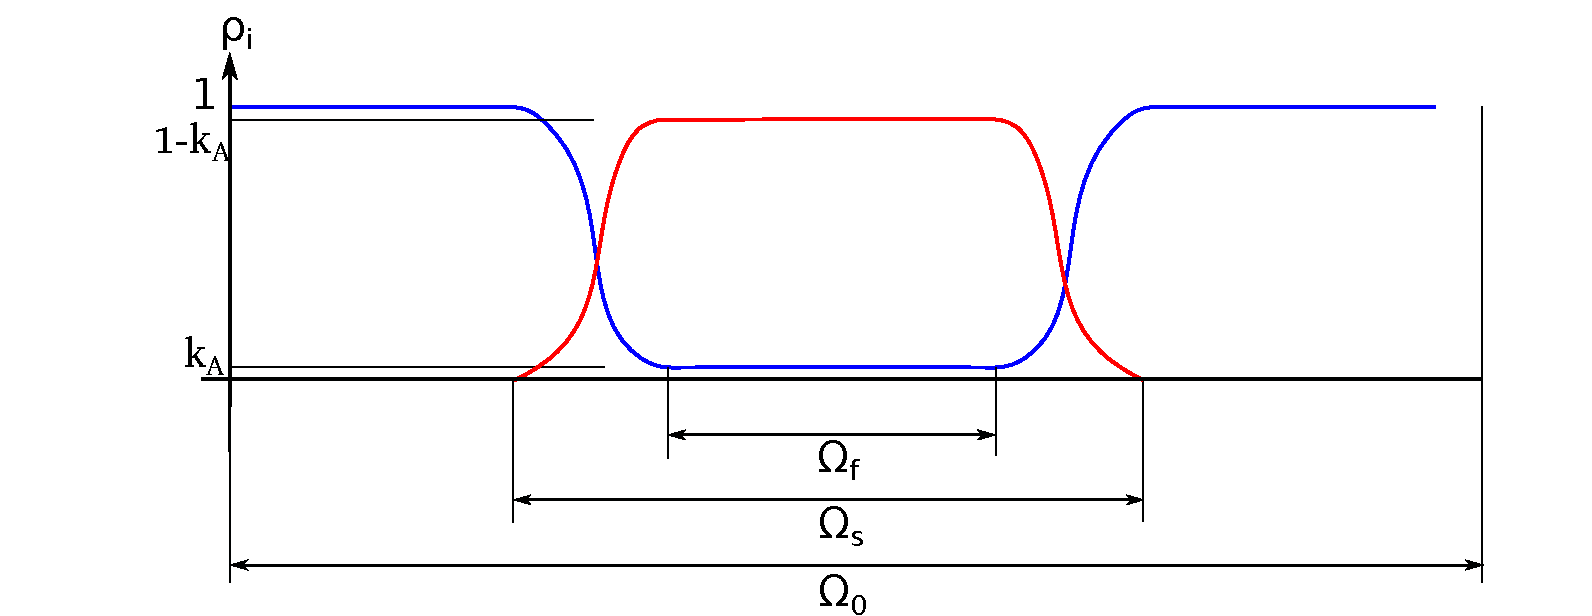
\includegraphics[scale=0.6,trim=0cm 0cm 0cm 0.0cm, clip=true]{Imagens/Cap6/ponderadora.pdf}	
	\caption{Função Ponderadora}
	\label{fig:constanteKa}
	%\vspace{-1em} % Diminui o espaço antes da figura
\end{figure}


\section{Método Arlequin clássico aplicado à problemas de escoamentos incompressíveis}

O método Arlequin vem sendo aplicado amplamente em diversos trabalhos da mecânica dos sólidos nas últimas décadas. Entretanto, no que diz respeito a materiais incompressíveis, pode-se citar mais recentemente o trabalho de \citeonline{JamondD:2013}, no qual os autores desenvolvem uma técnica para análise empregando elementos do tipo Taylor-Hood, que satisfazem a condição LBB. Essa metodologia é testada também para problemas descritos pelas equações de Stokes.

De acordo com os autores \citeonline{JamondD:2013} a principal dificuldade encontrada para aplicação do método Arlequin no contexto de materiais incompressíveis é que duas restrições devem ser aplicadas concomitantemente: a compatibilização dos campos de interesse na zona de colagem e a condição de incompressibilidade do material nessa mesma região. Os autores apontaram que a imposição da condição de incompressibilidade em ambos os modelos pode gerar problema de redundância, acarretando em um sistema algébrico associado singular.

A solução proposta pelos autores nesse trabalho foi a aplicação da condição de incompressibilidade em cada ponto do domínio computacional apenas uma vez. A metodologia consiste então da remoção da condição de incompressibilidade dos elementos total ou parcialmente encontrados na zona de colagem ($\gluingZone$) em um dos modelos. Indiferente do modelo eleito para a remoção da condição de incompressibilidade na zona de colagem, na zona livre, a condição de incompressibilidade é removida do modelo global. Deve-se destacar que no trabalho citado existem algumas recomendações com relação a estabilidade da metodologiam, como, por exemplo, a necessidade de existir pelo menos um elemento global na zona livre. Tal trabalho não explora as possíveis mudanças que acarretariam na estabilidade numérica em caso de sucessivas remoções e inclusões de condição de incompressibilidade no caso de um modelo local móvel.

Por esse motivo, e pelas pesquisas anteriores já realizadas pela presente autora e seu grupo de pesquisa, optou-se pela adoção de elementos estabilizados, os quais já foram retratos nos capítulos anteriores (Cap. \ref{capitulo:Cap2} e Cap. \ref{capitulo:Cap3}).

Para a construção do método de Arlequin clássico precisamos retomar às equações para um monomodelo apresentadas na seção \ref{capitulo:Cap2:FormaFraca} que representam a forma fraca discretizada espacialmente e estabilizada das equações da quantidade de movimento (Eq. \ref{eq:FinalSystem}) e da continuidade (Eq. \ref{eq:RC}). MUDAR AS EQUAÇÕES NO CAPÍTULO DE FLUIDOS PARA DEIXAR SEM O TERMO ALE INICIALMENTE. E ALTERAR AS EQUAÇÕES PARA FICAR COM A MESMA SIMBOLOGIA DE CONTORNO DAQUI.

Vamos considera os espaços de dimensão finita das funções tentativa que descrevem a velocidade ($\uArlequinSolution$) e a pressão ($\pArlequinSolution$) e seus respectivos espaços de funções testes $\uArlequinTest$ e $\pArlequinTest$, com $i = 0,1$ indicando o índice do modelo, definidos como:

\begin{align}
	\uArlequinSolution = \left\{\velocity_{i}^{h} \left . \right| \velocity_{i}^{h} \left(\cdot,t\right) \in (H^{1h}\left(\Omega_{i}\right), \velocity_{i}^{h} = \velocity_{Di}^{h} \textrm { em}  \ \boundary_{Di} \right\}
\end{align}

\begin{align}
	\pArlequinSolution = \left\{\press_{i}^{h} \left . \right| \press_{i}^{h} \left(\cdot\right) \in L^{2h}\left(\domain_{i}\right) \right\},
\end{align}

\begin{align}
	\uArlequinTest = \left\{\utest_{i}^{h} \left . \right| \utest_{i}^{h} \left(\cdot\right) \in H^{1h}\left(\domain_i\right), \utest_{i}^{h} = \mathbf{0} \textrm { em} \ \boundary_{D_i} \right\},
\end{align}

e,

\begin{align}
	\pArlequinTest = \pArlequinSolution.
\end{align}

Analogamente, os espaços das funções tentativas ($\lagSolution$) e teste ($\lagTest$) para o campo dos multiplicadores de Lagrange ($\lagrangeMultiplier$) são definidos como:

\begin{align}
	\lagSolution = \left\{\lagrangeMultiplier^{h} \left . \right| \lagrangeMultiplier^{h} \left(\cdot\right) \in H^{1h}\left(\domain_{c}\right) \right\},
\end{align}

\begin{align}
	\lagTest = \lagSolution.
\end{align}

A aplicação do operador de acoplamento $L^{2}$ à formulação clássica Arlequin consiste em dado os espaços tentativa e teste apresentados nas equações anteriores: Encontrar $(\uglobalh,\pglobalh,\ulocalh,\plocalh,\lagrangeMultiplierh)$ $\in$ $\uGlobalSolution \times \pGlobalSolution \times \uLocalSolution \times \pLocalSolution \times \lagSolution$ de maneira que  $\forall$ $\wglobalh \in \uGlobalTest$, $\qglobalh \in \pGlobalTest$, $\wlocalh \in \uLocalTest$, $\qlocalh \in \pLocalTest$, e $\forall$ $\lagrangeMultiplierWFh \in \lagTest$:

\begin{align}
	\begin{split}
		&\int_{\domain_0} \arlequinWFGlobal \density \wglobalh \cdot \frac{\partial\uglobalh}{\partial t} d\domain_{0} \\ 
		&\qquad+
		\int_{\domain_0} \arlequinWFGlobal \density \wglobalh \cdot  \left(\uglobalh \cdot \nabla\right) \uglobalh d\domain_{0}  \\ 
		&\qquad+	
		\int_{\domain_{0}} \arlequinWFGlobal \straintensor \left(\wglobalh\right) : \stresstensor \left(\uglobalh,\pglobalh\right)\ d\domain_{0} 
		 \\ 
		&\qquad+ \sum_{e=1}^{\nel} \int_{\domainE} \SUPG  \left(\left(\uglobalh \cdot \nabla \right) \wglobalh\right) \cdot \resMomGlobal\left(\uglobalh,\pglobalh \right)\  d\domain_{0} \\ 
		&\qquad+\sum_{e=1}^{\nel} \int_{\domainE} \LSIC \nabla \cdot \wglobalh \resPreGlobal 
		 \left(\uglobalh\right)\  d\domain_{0} \\
		 &\qquad+ \chi_{0} \int_{\domain_c} \wglobalh \cdot \lagrangeMultiplier^{h} d\domain_{c}  = \int_{\domain_0} \arlequinWFGlobal \density \wglobalh \cdot  \sbodyforce_{0}^{h} d\domain_{0} + \int_{\boundary_{0}} \arlequinWFGlobal \uglobalh \cdot \straction_{0}^{h}\ d\boundary_{0},
		\label{eq:FinalSystem0}
	\end{split}
\end{align}


\begin{align}
	\begin{split}
		&	\int_{\domain_{0}} \arlequinWFGlobal \qglobalh \nabla \cdot \uglobalh \ d\domain_{0} +
\sum_{e=1}^{\nel} \int_{\domainE} \PSPG \left(\frac{\nabla \qglobalh}{\density}\right) \cdot \resMomGlobal\left(\uglobalh,\pglobalh\right) \  d\domain_{0},
		\label{eq:RC0}
	\end{split}
\end{align}


\begin{align}
	\begin{split}
		&\int_{\domain_1} \arlequinWFLocal \density \wlocalh \cdot \frac{\partial\ulocalh}{\partial t} d\domain_{1} \\ 
		&\qquad+
		\int_{\domain_1} \arlequinWFLocal \density \wlocalh \cdot  \left(\ulocalh \cdot \nabla\right)\ulocalh d\domain_{1}  \\ 
		&\qquad+	
		\int_{\domain_{1}} \arlequinWFLocal \straintensor \left(\wlocalh\right) : \stresstensor \left(\ulocalh,\plocalh\right)\ d\domain_{1} 
		\\ 
		&\qquad+ \sum_{e=1}^{\nel} \int_{\domainE} \SUPG  \left( \right(\ulocalh \cdot \nabla \left) \wlocalh\right) \cdot \resMomLocal\left(\ulocalh,\plocalh \right)\  d\domain_{1} \\ 
		&\qquad+\sum_{e=1}^{\nel} \int_{\domainE} \LSIC \nabla \cdot \wlocalh \resPreLocal
		\left(\ulocalh\right)\  d\domain_{1} \\
		&\qquad+ \chi_{1} \int_{\domain_c} \wlocalh \cdot \lagrangeMultiplier^{h} d\domain_{c}  = \int_{\domain_1} \arlequinWFLocal \density \wlocalh \cdot  \sbodyforce_{1}^{h} d\domain_{1} + \int_{\boundary_{1}} \arlequinWFLocal \ulocalh \cdot \straction_{1}^{h}\ d\boundary_{1},
		\label{eq:FinalSystem1}
	\end{split}
\end{align}


\begin{align}
	\begin{split}
		&	\int_{\domain_{1}} \arlequinWFLocal \qlocalh \nabla \cdot \ulocalh \ d\domain_{1} +
		\sum_{e=1}^{\nel} \int_{\domainE} \PSPG \left(\frac{\nabla \qlocalh}{\density}\right) \cdot \resMomLocal \left(\ulocalh,\plocalh\right) \  d\domain_{1} = 0,\\
		\label{eq:RC1}
	\end{split}
\end{align}

\begin{align}
	\int_{\domain_{c}}  \lagrangeMultiplierWFh  \cdot \left(\uglobalh - \ulocalh \right) \ d\domain_{c}, 
		\label{eq:EqAcopla}
\end{align}



\noindent onde $\resMomI$ e ${\resPreI}$ são os resíduos da equação da quantidade de movimento e da equação da continuidade, com $i=0,1$, respectivamente, dados por:

\begin{align}
	\resMomI \left(\uArlqi,\pArlqi,\lagrangeMultiplierh \right)&=\arlequinWF_{i} \density\left(\frac{\partial\uArlqi}{\partial t}+ \left( \uArlqi \cdot \nabla \right) \uArlqi - \sbodyforce_i^{h}\right) - \arlequinWF_{i} \nabla \cdot \stresstensor\left(\uArlqi,\pArlqi\right)+ \chi_{i} \lagrangeMultiplierh \label{eq:resMomI},
\end{align}

\noindent

\begin{align}
	\resPreI\left(\uArlqi\right)&= \arlequinWF_{i} \nabla \cdot \uArlqi \label{eq:resPreI}, 
\end{align}

\noindent com $\chi_{i}$ descrito da maneira que se segue:


\begin{align}
	\chi_{i} = \begin{cases} (-1)^{i} \ se \ \mathbf{x} \in \domain_{c} \\
			   0 \ se \ \mathbf{x} \notin \domain_{c}. \end{cases}						. 
\end{align}

O problema descrito pelas equações \ref{eq:FinalSystem0} à \ref{eq:EqAcopla} descreve à versão clássica do método de Arlequin para o problema de Navier-Stokes estabilizado pela técnica PSPG/SUPG. Matematicamente trata-se de um problema de ponto de sela decorrente de uma formulação mista. Entretanto, desde que a condição LBB seja satisfeita, existe solução para o problema e ela é única. 

Em \citeonline{GuidaultAndBelytschko2007} pode-se encontrar uma vasta análise matemática a cerca das questões relacionadas com estabilidade, convergência e relevância do método. Nesta pesquisa, os autores relatam, por exemplo, a necessidade de emprego de funções ponderadoras contínuas quando utilizado o operador de acoplamento $L^{2}$, tal caso não ocorre com o operador de acoplamento $H^{1}$. Além disso,  os autores destacam que espaços muito refinados para os acopladores de Lagrange podem levar a uma solução não convergente, independente do tipo de operador de acoplamento. Este problema ocorre devido a forte dependência da discretização do modelo global na solução.

O problema descrito no método Arlequin clássico é análogo a formulação mista em elementos finitos para escoamentos incompressíveis, que limita a escolha das funções aproximadoras para o campo de velocidade e pressão. No caso da mecânica dos fluidos, conforme apresentado no Cap. \ref{capitulo:Cap2}, uma forma de superar esta restrição LBB é o uso de métodos estabilizados como o PSPG. Seguindo essa mesma filosofia,  \citeonline{FernandesEtAll:2020} introduzem uma técnica de estabilização consistente que será apresentada na seguinte seção. 

\section{Método Arlequin estabilizado aplicado à problemas de escoamentos incompressíveis}


Com intuito de superar a condição LBB para o problema de Arlequin, \citeonline{FernandesEtAll:2020} desenvolvem uma técnica de estabilização consistente baseada em resíduo. Para isso, introduz-se uma parcela adicional à equação dos campos de multiplicadores de Lagrange, que leva em conta o gradiente de $\lagrangeMultiplierWFh$ e o resíduo da equação da quantidade de movimento:

\begin{align}
	\sum_{e=1}^{\nel} \int_{\domainE_{c}} \frac{\tauArlequinGlobal}{\rho} \nabla \lagrangeMultiplierWFh : \nabla \resMomGlobal\left(\uglobalh,\pglobalh \right) \ d\domain_{c} - 
	\sum_{e=1}^{\nel} \int_{\domainE_{c}} \frac{\tauArlequinLocal}{\rho} \nabla \lagrangeMultiplierWFh : \nabla \resMomLocal\left(\ulocalh,\plocalh \right) \ d\domain_{c},
\end{align}

\noindent sendo $\tauArlequinGlobal$ e $\tauArlequinLocal$ parâmetros de estabilização, respectivamente da malha global e local. A obtenção destes parâmetros será abordada na subseção seguinte. 

Dessa forma, pode-se definir a solução do problema de Navier-Stokes para escoamentos incompressíveis utilizando a técnica de Arlequin estabilizada da seguinte forma: Encontrar $(\uglobalh,\pglobalh,\ulocalh,\plocalh,\lagrangeMultiplierh)$ $\in$ $\uGlobalSolution \times \pGlobalSolution \times \uLocalSolution \times \pLocalSolution \times \lagSolution$ de maneira que  $\forall$ $\wglobalh \in \uGlobalTest$, $\qglobalh \in \pGlobalTest$, $\wlocalh \in \uLocalTest$, $\qlocalh \in \pLocalTest$,   e $\forall$ $\lagrangeMultiplierWFh \in \lagTest$:

\begin{align}
	\begin{split}
		&\int_{\domain_0} \arlequinWFGlobal \density \wglobalh \cdot \frac{\partial\uglobalh}{\partial t} d\domain_{0} +
		\int_{\domain_0} \arlequinWFGlobal \density \wglobalh \cdot  \left(\uglobalh \cdot \nabla\right)\uglobalh d\domain_{0}  \\ 
		&\qquad+	
		\int_{\domain_{0}} \arlequinWFGlobal \straintensor \left(\wglobalh\right) : \stresstensor \left(\uglobalh,\pglobalh\right)\ d\domain_{0} 
		\\ 
		&\qquad+ \sum_{e=1}^{\nel} \int_{\domainE} \SUPG  \left(\left(\uglobalh \cdot \nabla \right) \wglobalh\right) \cdot \resMomGlobal\left(\uglobalh,\pglobalh \right)\  d\domain_{0} \\ 
		&\qquad+\sum_{e=1}^{\nel} \int_{\domainE} \LSIC \nabla \cdot \wglobalh \resPreGlobal 
		\left(\uglobalh\right)\  d\domain_{0} \\
		&\qquad+ \chi_{0} \int_{\domain_c} \wglobalh \cdot \lagrangeMultiplier^{h} d\domain_{c}  = \int_{\domain_0} \arlequinWFGlobal \density \wglobalh \cdot  \sbodyforce_{0}^{h} d\domain_{0} + \int_{\boundary_{0}} \arlequinWFGlobal \uglobalh \cdot \straction_{0}^{h}\ d\boundary_{0}, 
		\label{eq:FinalSystem0est}
	\end{split}
\end{align}


\begin{align}
	\begin{split}
		&	\int_{\domain_{0}} \arlequinWFGlobal \qglobalh \nabla \cdot \uglobalh \ d\domain_{0} +
		\sum_{e=1}^{\nel} \int_{\domainE} \PSPG \left(\frac{\nabla \qglobalh}{\density}\right) \cdot \resMomGlobal\left(\uglobalh,\pglobalh\right) \  d\domain_{0} = 0, 
		\label{eq:RC0est}
	\end{split}
\end{align}


\begin{align}
	\begin{split}
		&\int_{\domain_1} \arlequinWFLocal \density \wlocalh \cdot \frac{\partial\ulocalh}{\partial t} d\domain_{1} +
		\int_{\domain_1} \arlequinWFLocal \density \wlocalh \cdot  \left(\ulocalh \cdot \nabla\right)\ulocalh d\domain_{1}  \\ 
		&\qquad+	
		\int_{\domain_{1}} \arlequinWFLocal \straintensor \left(\wlocalh\right) : \stresstensor \left(\ulocalh,\plocalh\right)\ d\domain_{1} 
		\\ 
		&\qquad+ \sum_{e=1}^{\nel} \int_{\domainE} \SUPG  \left( \right(\ulocalh \cdot \nabla \left) \wlocalh\right) \cdot \resMomLocal\left(\ulocalh,\plocalh \right)\  d\domain_{1} \\ 
		&\qquad+\sum_{e=1}^{\nel} \int_{\domainE} \LSIC \nabla \cdot \wlocalh \resPreLocal
		\left(\ulocalh\right)\  d\domain_{1} \\
		&\qquad+ \chi_{1} \int_{\domain_c} \wlocalh \cdot \lagrangeMultiplier^{h} d\domain_{c}  = \int_{\domain_1} \arlequinWFLocal \density \wlocalh \cdot  \sbodyforce_{1}^{h} d\domain_{1} + \int_{\boundary_{1}} \arlequinWFLocal \ulocalh \cdot \straction_{1}^{h}\ d\boundary_{1}, 
		\label{eq:FinalSystem1est}
	\end{split}
\end{align}


\begin{align}
	\begin{split}
		&	\int_{\domain_{1}} \arlequinWFLocal \qlocalh \nabla \cdot \ulocalh \ d\domain_{1}+
		\sum_{e=1}^{\nel} \int_{\domainE} \PSPG \left(\frac{\nabla \qlocalh}{\density}\right) \cdot \resMomLocal \left(\ulocalh,\plocalh\right) \  d\domain_{1} = 0, 
		\label{eq:RC1est}
	\end{split}
\end{align}


\begin{align}
	\begin{split}
	&\int_{\domain_{c}}  \lagrangeMultiplierWFh  \cdot \left(\uglobalh - \ulocalh \right) \ d\domain_{c} + \sum_{e=1}^{\nel} \int_{\domainE_{c}} \frac{\tauArlequinGlobal}{\rho} \nabla \lagrangeMultiplierWFh : \nabla \resMomGlobal\left(\uglobalh,\pglobalh\right) \ d\domain_{c}  \\
	&\qquad-\sum_{e=1}^{\nel} \int_{\domainE_{c}} \frac{\tauArlequinLocal}{\rho} \nabla \lagrangeMultiplierWFh : \nabla \resMomLocal \ d\domain_{c},
	\label{eq:EqAcoplaest}
\end{split}
\end{align}

\noindent com os resíduos $\resMomI$ e $\resPreI$ escritos conforme as Eq. \ref{eq:resMomI} e Eq .\ref{eq:resPreI}.

O sistema resultante pode ser reescrito em notação matricial como:

\begin{align}
	\begin{bmatrix}
		\mathbf{K_{0}} & \mathbf{0} & \hat{\mathbf{L}_{0}} \\
		\mathbf{0} & \mathbf{K_{1}} & - \hat{\mathbf{L}_{1}} \\
		\mathbf{L}_{0}^{T} & -\mathbf{L}_{1}^{T} & \mathbf{E}
	\end{bmatrix}
	\begin{bmatrix}
		\mathbf{U_{0}} \\
		\mathbf{U_{1}} \\
		\lagrangeMultiplier
	\end{bmatrix}
	&=
	\begin{bmatrix}
		\mathbf{F_{0}} \\
		\mathbf{F_{1}} \\
		\mathbf{F_{\lagrangeMultiplier}}
	\end{bmatrix}.
	\label{eq:sistema_linear}
\end{align}	

Como poderia chamar essas matrizes?

Note que na estabilização Arlequin baseada no resíduo (RBSAM) não existem elementos zeros na diagonal da matriz, diferente do mesmo problema na formulação clássica Arlequin. No trabalho de \citeonline{FernandesEtAll:2020} pode-se encontrar a análise de estabilidade dessa técnica e testes numéricos que avaliam o condicionamento do sistema algébrico e a convergência do método.

O problema de Arlequin não linear apresentado nas equações: Eq. \ref{eq:FinalSystem0est} à \ref{eq:EqAcoplaest} pode ser reescrito em sua forma semi-discreta residual para $i=0,1$, da seguinte maneira:

\begin{align}
	\begin{split}
		&\mathbf{R}_{M,i} = \int_{\domain_i} \arlequinWF_{i} \density \wArlqi \cdot \frac{\partial\uArlqi}{\partial t} d\domain_{i} +
		\int_{\domain_i} \arlequinWF_{i} \density \wArlqi \cdot  \left(\uArlqi \cdot \nabla\right)\uArlqi d\domain_{i}  \\ 
		&\qquad+	
		\int_{\domain_{i}} \arlequinWF_{i} \straintensor \left(\wArlqi\right) : \stresstensor \left(\uArlqi,\pArlqi\right)\ d\domain_{i} 
		\\ 
		&\qquad+ \sum_{e=1}^{\nel} \int_{\domainE} \SUPG  \left( \right(\uArlqi \cdot \nabla \left) \wArlqi\right) \cdot \resMomI \left(\uArlqi,\pArlqi \right)\  d\domain_{i} \\ 
		&\qquad+\sum_{e=1}^{\nel} \int_{\domainE} \LSIC \nabla \cdot \wArlqi \resPreI
		\left(\uArlqi\right)\  d\domain_{i} \\
		&\qquad+ \chi_{i} \int_{\domain_c} \wArlqi \cdot \lagrangeMultiplier^{h} d\domain_{c} - \int_{\domain_i} \arlequinWF_{i} \density \wArlqi \cdot  \sbodyforce_{i}^{h} d\domain_{i} - \int_{\boundary_{i}} \arlequinWF_{i} \uArlqi \cdot \straction_{i}^{h}\ d\boundary_{i},
		\label{eq:ResidualMomentum}
	\end{split}
\end{align}


\begin{align}
	\begin{split}
		&\mathbf{R}_{C,i} = \int_{\domain_{i}} \arlequinWF_{i} \qArlqi \nabla \cdot \uArlqi \ d\domain_{i} +
		\sum_{e=1}^{\nel} \int_{\domainE} \PSPG \left(\frac{\nabla \qArlqi }{\density}\right) \cdot \resMomI \left(\uArlqi,\pArlqi \right) \  d\domain_{i},
		\label{eq:ResidualContinum}
	\end{split}
\end{align}

\begin{align}
	\begin{split}
		&\mathbf{R}_{L} = \int_{\domain_{c}}  \lagrangeMultiplierWFh  \cdot \left(\uglobalh - \ulocalh \right) \ d\domain_{c} + \sum_{e=1}^{\nel} \int_{\domainE_{c}} \frac{\tauArlequinGlobal}{\rho} \nabla \lagrangeMultiplierWFh : \nabla \resMomGlobal\left(\uglobalh,\pglobalh\right) \ d\domain_{c}\\
		&\qquad - \sum_{e=1}^{\nel} \int_{\domainE_{c}} \frac{\tauArlequinLocal}{\rho} \nabla \lagrangeMultiplierWFh : \nabla \resMomLocal\left(\ulocalh,\plocalh\right) \ d\domain_{c}.
		\label{eq:ResidualLagrange}
	\end{split}
\end{align}

Considerando $\Acceleration_{i}$, $\Velocity_{i}$, $\Press_i$ e $\LagrangeMultiplier$ os vetores nodais dos graus de liberdade respectivos a aceleração, velocidade, pressão e multiplicadores de Lagrange, pode-se escrever o problema semidiscreto da DFC como: Determinar $\Acceleration_0$, $\Velocity_0$, $\Press_0$,$\Acceleration_1$, $\Velocity_1$, $\Press_1$ e $\LagrangeMultiplier$ de maneira que:

\begin{align}
	\mathbf{R}_{M,0}(\Acceleration_0,\Velocity_0,\Press_0,\LagrangeMultiplier) = \mathbf{0}, \label{eq:NLinear1}
\end{align}

\begin{align}
	\mathbf{R}_{C,0}(\Acceleration_0,\Velocity_0,\Press_0,\LagrangeMultiplier) = \mathbf{0},
\end{align}

\begin{align}
	\mathbf{R}_{M,1}(\Acceleration_1,\Velocity_1,\Press_1,\LagrangeMultiplier) = \mathbf{0},
\end{align}

\begin{align}
	\mathbf{R}_{C,1}(\Acceleration_1,\Velocity_1,\Press_1,\LagrangeMultiplier) = \mathbf{0},
\end{align}

\begin{align}
	\mathbf{R}_{L}(\Acceleration_0,\Velocity_0,\Press_0,\Acceleration_1,\Velocity_1,\Press_1,\LagrangeMultiplier) = \mathbf{0}. \label{eq:NLinear5}
\end{align}


\subsection{Integração Temporal}


Quanto ao procedimento de integração temporal, utilizou-se o método $\alpha$-generalizado. Conforme a metodologia apresentado na seção \ref{sec:IntegTemp}, para a solução do sistema de equações não lineares compostas por Eq. \eqref{eq:NLinear1} à Eq. \eqref{eq:NLinear5} utiliza-se o método de Newton-Raphson. A solução resulta em uma etapa preditiva e outra iterativa corretiva.

Na etapa preditiva, conhecida a solução em um passo de tempo $n$, prediz-se a solução no passo seguinte ($n+1$) através das seguintes relações:

\begin{align}
	\Acceleration_{0(n+1)}^{0} = \frac{\gamma-1}{\gamma}\Acceleration_{0(n)} \label{eq:PredArlq1},
\end{align}

\begin{align}
	\Velocity_{0(n+1)}^{0} = \Velocity_{0(n)}, \label{eq:PredArlq2}
\end{align}

\begin{align}
	\Press_{0(n+1)}^{0} = \Press_{0(n)},\label{eq:PredArlq3}
\end{align}

\begin{align}
	\Acceleration_{1(n+1)}^{0} = \frac{\gamma-1}{\gamma}\Acceleration_{1(n)} \label{eq:PredArlq4},
\end{align}

\begin{align}
	\Velocity_{1(n+1)}^{0} = \Velocity_{1(n)}, \label{eq:PredArlq5}
\end{align}

\begin{align}
	\Press_{1(n+1)}^{0} = \Press_{1(n)},\label{eq:PredArlq6}
\end{align}

\begin{align}
	\LagrangeMultiplier_{(n+1)}^{0} = \LagrangeMultiplier_{(n)},\label{eq:PredArlq7}
\end{align}

\noindent onde o superíndice $0$ representa a iteração de número zero, enquanto que os subíndices $0$ e $1$ representam as variáveis do modelo global e local respectivamente.

Na etapa iterativa corretiva, itera-se sobre a Eq. \eqref{eq:NLinear1} à Eq. \eqref{eq:NLinear5} até que elas sejam satisfeitas, seja através de uma tolerância prescrita, ou até que se alcance uma quantidade máxima de iterações pré-estabelecida. A etapa iterativa corretiva é constituida por três fases. A fase 1 consiste em determinar os valores no instante intermediário para as variáveis nodais na iteração $i$:

\begin{align}
	\Acceleration_{0({n+\alpham})}^{i} = \Acceleration_{0(n)} + \alpham \left( \Acceleration_{0(n+1)}^{i} - \Acceleration_{0(n)} \right), \label{eq:Inter1}\\
	\Velocity_{0(n+\alphaf)}^{i} = \Velocity_{0(n)} + \alphaf \left( \Velocity_{0(n+1)}^{i} - \Velocity_{0(n)} \right), \label{eq:Inter2}\\
	\Press_{0(n+1)}^{i} = \Press_{0(n+1)}^{i}, \label{eq:Inter3} \\
	\Acceleration_{1(n+\alpham)}^{i} = \Acceleration_{1(n)} + \alpham \left( \Acceleration_{1(n+1)}^{i} - \Acceleration_{1(n)} \right), \label{eq:Inter4}\\
	\Velocity_{1(n+\alphaf)}^{i} = \Velocity_{1(n)} + \alphaf \left( \Velocity_{1(n+1)}^{i} - \Velocity_{1(n)} \right), \label{eq:Inter5}\\
	\Press_{1(n+1)}^{i} = \Press_{1(n+1)}^{i},\label{eq:Inter6} \\
	\LagrangeMultiplier_{(n+1)}^{i} = \LagrangeMultiplier_{(n+1)}^{i}. \label{eq:Inter7}
\end{align}

Na fase 2, com os valores intermediários das variáveis nodais resolve-se o sistema linear resultante da linearização das equações Eq. \eqref{eq:NLinear1} à Eq. \eqref{eq:NLinear1} com respeito às variáveis de interesse $\Acceleration_{0(n+1)}$, $\Press_{0(n+1)}$,  $\Acceleration_{1(n+1)}$, $\Press_{1(n+1)}$ e $\LagrangeMultiplier_{(n+1)}$:

\begin{align}
	\begin{bmatrix}
		\frac{\partial\mathbf{R}_{M,0}}{\partial\Acceleration_{0(n+1)}^{i}} & \frac{\partial\mathbf{R}_{M,0}}{\partial\Press_{0(n+1)}^{i}} & \mathbf{0} & \mathbf{0} & \frac{\partial\mathbf{R}_{M,0}}{\partial\LagrangeMultiplier_{(n+1)}^{i}} \\
		\frac{\partial\mathbf{R}_{C,0}}{\partial\Acceleration_{0(n+1)}^{i}} & \frac{\partial\mathbf{R}_{C,0}}{\partial\Press_{0(n+1)}^{i}} & \mathbf{0} & \mathbf{0} & \frac{\partial\mathbf{R}_{C,0}}{\partial\LagrangeMultiplier_{(n+1)}^{i}} \\
		 \mathbf{0} & \mathbf{0} & \frac{\partial\mathbf{R}_{M,1}}{\partial\Acceleration_{1(n+1)}^{i}} & \frac{\partial\mathbf{R}_{M,1}}{\partial\Press_{1(n+1)}^{i}} & \frac{\partial\mathbf{R}_{M,1}}{\partial\LagrangeMultiplier_{(n+1)}^{i}} \\
		 \mathbf{0} & \mathbf{0} & \frac{\partial\mathbf{R}_{C,1}}{\partial\Acceleration_{1(n+1)}^{i}} & \frac{\partial\mathbf{R}_{C,1}}{\partial\Press_{1(n+1)}^{i}} & \frac{\partial\mathbf{R}_{C,1}}{\partial\LagrangeMultiplier_{(n+1)}^{i}} \\
		  \frac{\partial\mathbf{R}_{L}}{\partial\Acceleration_{0(n+1)}^{i}} & \frac{\partial\mathbf{R}_{L}}{\partial\Press_{0(n+1)}^{i}} & \frac{\partial\mathbf{R}_{L}}{\partial\Acceleration_{1(n+1)}^{i}} & \frac{\partial\mathbf{R}_{L}}{\partial\Press_{1(n+1)}^{i}} & \frac{\partial\mathbf{R}_{L}}{\partial\LagrangeMultiplier_{(n+1)}^{i}}
	\end{bmatrix}
	\begin{bmatrix}
		\Delta\Acceleration_{0(n+1)}^{i} \\
		\Delta\Press_{0(n+1)}^{i} \\
		\Delta\Acceleration_{1(n+1)}^{i} \\
		\Delta\Press_{1(n+1)}^{i} \\
		\LagrangeMultiplier_{(n+1)}^{i}
	\end{bmatrix}
	&=
	\begin{bmatrix}
		-\mathbf{R}_{M,0} \\
		-\mathbf{R}_{C,0} \\
		-\mathbf{R}_{M,1} \\
		-\mathbf{R}_{C,1} \\
		-\mathbf{R}_{L}
	\end{bmatrix}
	\label{eq:sistema_linear_Arlq}
\end{align}	

Atualiza-se então na fase 3 a solução através das seguintes relações:

\begin{align}
	\Acceleration_{0(n+1)}^{i+1} = \Acceleration_{0(n+1)}^{i} + \Delta\Acceleration_{0(n+1)}^{i}, \label{eq:up1} \\ 
	\Velocity_{0(n+1)}^{i+1} = \Velocity_{0(n+1)}^{i} + \Delta\Velocity_{0(n+1)}^{i},\label{eq:up2}\\
	\Press_{0(n+1)}^{i+1} = \Press_{0(n+1)}^{i} + \Delta\Press_{0(n+1)}^{i}, \label{eq:up3} \\
	\Acceleration_{1(n+1)}^{i+1} = \Acceleration_{1(n+1)}^{i} + \Delta\Acceleration_{1(n+1)}^{i}, \label{eq:up4} \\ 
	\Velocity_{1(n+1)}^{i+1} = \Velocity_{1(n+1)}^{i} + \Delta\Velocity_{1(n+1)}^{i},\label{eq:up5}\\
	\Press_{1(n+1)}^{i+1} = \Press_{0(n+1)}^{i} + \Delta\Press_{1(n+1)}^{i}, \label{eq:up6} \\
	\LagrangeMultiplier_{1(n+1)}^{i+1} = \LagrangeMultiplier_{0(n+1)}^{i} + \Delta\LagrangeMultiplier_{1(n+1)}^{i}. \label{eq:up7}
\end{align}

Na utilização do método $\alpha$-generalizado as integrais das equações são avaliadas no instante $t = t_{n+\alpha_{f}}$. As relações entre velocidade e aceleração, e os parâmetros utilizados pelo método podem ser consultados na Seção \ref{sec:IntegTemp}.


\subsection{Parâmetro de estabilização para técnica RBSAM}

No método Arlequin existe a necessidade de definição do paramêtro de estabilização $\tauArlequin$. Este parâmetro deve possuir valor suficiente para estabilizar os campos de multiplicadores de Lagrange, sem, no entanto, comprometer a convergência do método. 

Para a definição de $\tauArlequin$ tomou-se como referência os trabalhos de \citeonline{TezduyarO:2000} e \citeonline{TezduyarS:2003} nos quais se apresenta uma vasta quantidade de informação a cerca da obtenção dos parâmetros de estabilização das equações da DFC ($\SUPG$, $\PSPG$, $\LSIC$). 
 
Propõe-se como critério a obtenção de termos de estabilização com magnitude próxima aos termos da equação de acoplamento, através da utilização de normas vetoriais. Este parâmetro será definido para cada um dos modelos como:

\begin{align}
	\tauArlequini = \left(\frac{1}{\left(\tau_{A_i}\right)^{2}} + \frac{1}{\left(\tau_{B_i}\right)^{2}} +  \frac{1}{\left(\tau_{C_i}\right)^{2}} + 
	\frac{1}{\left(\tau_{D_i}\right)^{2}} +
	\frac{1}{\left(\tau_{E_i}\right)^{2}}
	\right)^{-\frac{1}{2}},
\end{align}

\noindent com $i=0,1$ definindo o modelo global e local respectivamente e:

\begin{align}
	\tau_{A_{i}} = \left(\frac{1}{\left(\tau_{A_i^{0}}\right)^{2} + \left(\tau_{A_i^{1}}\right)^{2}} \right)^{-\frac{1}{2}}, \label{eq:tAi}
\end{align}

\begin{align}
	\tau_{B_{i}} = \left(\frac{1}{\left(\tau_{B_i^{0}}\right)^{2} + \left(\tau_{B_i^{1}}\right)^{2}} \right)^{-\frac{1}{2}},
\end{align}

\begin{align}
	\tau_{C_{i}} = \left(\frac{1}{\left(\tau_{C_i^{0}}\right)^{2} + \left(\tau_{C_i^{1}}\right)^{2}} \right)^{-\frac{1}{2}},
\end{align}

\begin{align}
	\tau_{D_{i}} = \left(\frac{1}{\left(\tau_{D_i^{0}}\right)^{2} + \left(\tau_{D_i^{1}}\right)^{2}} \right)^{-\frac{1}{2}},
\end{align}

\begin{align}
	\tau_{E_{i}} = \left(\frac{1}{\left(\tau_{E_i^{0}}\right)^{2} + \left(\tau_{E_i^{1}}\right)^{2}} \right)^{-\frac{1}{2}},\label{eq:tEi}
\end{align}

\noindent sendo as variáveis das equacões \refeq{eq:tAi} à \refeq{eq:tAi} as seguintes normas vetoriais:

\begin{align}
	\tau_{A_i^{0}} = \frac{|| \mathbf{M_{\lambda_0}} || }{||\mathbf{t_{i}} ||}; \ \ \ \ \  & \tau_{A_i^{1}} = \frac{|| \mathbf{M_{\lambda_1}} || }{||\mathbf{t_{i}} ||}  ,
\end{align}


\begin{align}
	\tau_{B_i^{0}} = \frac{|| \mathbf{M_{\lambda_0}} || }{||\mathbf{j_{i}} ||}; \ \ \ \ \  &  \tau_{B_i^{1}} = \frac{|| \mathbf{M_{\lambda_1}} || }{||\mathbf{j_{i}} ||}, 
\end{align}

\begin{align}
	\tau_{C_i^{0}} = \frac{|| \mathbf{M_{\lambda_0}} || }{||\mathbf{k_{i}} ||}; \ \ \ \ \  & \tau_{C_i^{1}} = \frac{|| \mathbf{M_{\lambda_1}} || }{||\mathbf{k_{i}} ||},
\end{align}


\begin{align}
	\tau_{D_i^{0}} = \frac{|| \mathbf{M_{\lambda_0}} || }{||\mathbf{p_{i}} ||}; \ \ \ \ \  & \tau_{D_i^{1}} = \frac{|| \mathbf{M_{\lambda_1}} || }{||\mathbf{p_{i}} ||}, 
\end{align}


\begin{align}
	\tau_{E_i^{0}} = \frac{|| \mathbf{M_{\lambda_0}} || }{||\mathbf{\boundary_{i}} ||} \ \ \ \ \  & \tau_{E_i^{1}} = \frac{|| \mathbf{M_{\lambda_1}} || }{||\mathbf{\boundary_{i}} ||}.
\end{align}

Por fim, os vetores em questão, são definidos através das seguintes relações:


\begin{align}
	\mathbf{M_{\lambda_0}} = \int_{\domain_{c}^{e}} N_{k} \cdot \mathbf{u_{0}^{h}} d\domain_{c}^{e},
\end{align}

\begin{align}
	\mathbf{M_{\lambda_1}} = - \int_{\domain_{c}^{e}} N_{k} \cdot \mathbf{u_{1}^{h}} d\domain_{c}^{e},
\end{align}

\begin{align}
	\mathbf{t_{i}} = \int_{\domain_{c}^{e}} \nabla N_{k} : \arlequinWF_{i} \nabla \left( \left( \uArlqi \cdot  \nabla \right) \uArlqi \right)  d\domain_{c}^{e},
\end{align}

\begin{align}
	\mathbf{j_{i}} = \int_{\domain_{c}^{e}} \nabla N_{k} :  \arlequinWF_{i} \nabla \left(\frac{\partial\uArlqi}{\partial t}  \right)  d\domain_{c}^{e},
\end{align}

\begin{align}
	\mathbf{k_{i}} = \int_{\domain_{c}^{e}} \nabla^{2} N_{k} : \arlequinWF_{i} 2 \mu \nabla \cdot \straintensor \left(\uArlqi\right)    d\domain_{c}^{e},
\end{align}

\begin{align}
	\mathbf{p_{i}} = \int_{\domain_{c}^{e}} \nabla N_{k} : \arlequinWF_{i} \nabla \left(-\nabla p_i^h\right)    d\domain_{c}^{e},
\end{align}

\begin{align}
	\mathbf{\boundary_{i}} = \int_{\domain_{c}^{e}} \nabla N_{k} : \nabla \left(\chi (i) \lagrangeMultiplierh\right)    d\domain_{c}^{e},
\end{align}


\noindent com $k$ representando o índice dos graus de liberdade do campo de multiplicadores de Lagrange.


\section{Superposição de modelos móveis}

As equações Eq. \ref{eq:FinalSystem0est} à \ref{eq:EqAcoplaest} resolvem problemas de escoamentos incompressíveis em uma discretização Euleriana. Entretanto, como têm-se como alvo à movimentação do domínio local do fluido (ver Fig. \ref{fig:ArlquinMóvel}) para acomodar a movimentação da estrutura em problemas de IFE ou representar a movimentação de um objeto imerso na DFC, faz-se o uso de uma descrição Lagrangiana-Euleriana Arbitrária (ALE) no modelo local ($\localModel$) enquanto que o domínio global ($\globalModel$) mantém-se fixo e com descrição Euleriana. 

Para o entendimento da metodologia de superposição de modelos móveis em um esquema Euleriano-ALE, pode-se analisar a Fig. \ref{fig:ArlquinMóvel}. Nela, pode-se observar a mudança de configuração dos modelos de fluido do passo $t_n$ para o passo $t_{n+1}$. Nota-se que o modelo global mantém sua geometria inalterada na mudança de passo de tempo, enquanto que o modelo local é movimentado para representar uma nova localização de um objeto imerso. Vale ressaltar que o contorno do domínio do modelo local ($\localModel$) é conhecido em $t_n$ e em $t_{n+1}$, e que a zona de superposição $\overlappingZone$ é definida em diferentes posições em cada instante.


Para análise de domínios móveis do tipo Euleriano-ALE, a Eq. \ref{eq:FinalSystem1est} será reescrita, levando-se em consideração as definições apresentadas na Seção \ref{Capítulo2:ALE}, como:


\begin{align}
	\begin{split}
		&\int_{\domain_1} \arlequinWFLocal \density \wlocalh \cdot \frac{\partial\ulocalh}{\partial t} d\domain_{1} \\ 
		&\qquad+
		\int_{\domain_1} \arlequinWFLocal \density \wlocalh \cdot  \left(\left(\ulocalh - \velocityALEh_{1}\right) \cdot \nabla\ulocalh\right) d\domain_{1}  \\ 
		&\qquad+	
		\int_{\domain_{1}} \arlequinWFLocal \straintensor \left(\wlocalh\right) : \stresstensor \left(\ulocalh,\plocalh\right)\ d\domain_{1} 
		\\ 
		&\qquad+ \sum_{e=1}^{\nel} \int_{\domainE} \SUPG  \left( \right(\ulocalh \cdot \nabla \left) \wlocalh\right) \cdot \resMomLocal\left(\ulocalh,\plocalh \right)\  d\domain_{1} \\ 
		&\qquad+\sum_{e=1}^{\nel} \int_{\domainE} \LSIC \nabla \cdot \wlocalh \resPreLocal
		\left(\ulocalh\right)\  d\domain_{1} \\
		&\qquad+  \chi_{1} \int_{\domain_c} \wlocalh \cdot \lagrangeMultiplier^{h} d\domain_{c}  = \int_{\domain_1} \arlequinWFLocal \density \wlocalh \cdot  \sbodyforce_{1}^{h} d\domain_{1} + \int_{\boundary_{1}} \arlequinWFLocal \ulocalh \cdot \straction_{1}^{h}\ d\boundary_{1},
		\label{eq:QtdeMovArlqALE}
	\end{split}
\end{align}

\noindent e o resíduo apresentado na Eq. \ref{eq:resMomI} ficará reescrito para i = 1, como:


\begin{align}
	\resMomLocal \left(\ulocalh,\plocalh,\lagrangeMultiplierh \right)&=\arlequinWF_{1} \density\left(\frac{\partial\ulocalh}{\partial t}+ \left(\ulocalh - \velocityALEh_{1}\right) \cdot \nabla\ulocalh  - \sbodyforce_1^{h}\right) - \arlequinWF_{1} \nabla \cdot \stresstensor\left(\ulocalh,\plocalh,\right)+ \chi_{1} \lagrangeMultiplierh \label{eq:resMomARLQALE}.
\end{align}

Além da consideração da descrição ALE para o modelo local, deve-se ressaltar que a função ponderadora $\arlequinWF_{i}$ passa a ser uma variável temporal, ou seja, $\arlequinWF_{i}(t)$ para o modelo global, visto que a zona de superposição $\overlappingZone$ é definida em diferentes posições em cada instante de tempo. Dessa forma, a integração temporal utilizando o método $\alpha$-generalizado deve considerar essa variação através da seguinte interpolação no tempo intermediário:

\begin{align}
	\arlequinWF_{0(n+\alphaf)} = \arlequinWF_{0(n)} + \alphaf(\arlequinWF_{0(n+1)} - \arlequinWF_{0(n)}).
\end{align}

\begin{figure}[htb!]
	\centering 
	{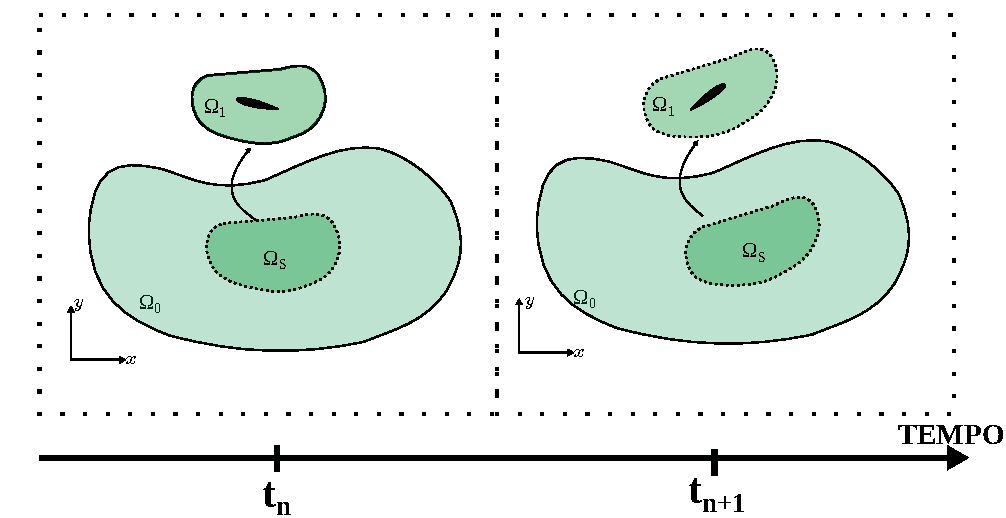
\includegraphics[scale=1.0,trim=0cm 0cm 0cm 0cm, clip=true]{Imagens/Cap6/dominioArlequinMoving.pdf}}	
	\caption{Domínio Arlequin móvel}
	\label{fig:ArlquinMóvel}
\end{figure}

A solução de modelos móveis requer a utilização de uma técnica adequada para movimentação da malha local. A técnica utilizada nesse trabalho é conhecida como MJBS (Mesh-Jacobian Based Stiffening) introduzida por \citeonline{TezduyarBSJ:1992f} e será abordada na Seção \ref{section:MovMalha}.


\section{Implementação Computacional}


Previamente à explicação a cerca da implementação computacional, é importante indicar que o campo dos multiplicadores de Lagrange é definido neste estudo na malha local. Tal escolha ocorre pelo fato de que mesmo em problemas em que se tenham grandes deslocamentos, a quantidade de elementos locais da zona de superposição permanece inalterada, fazendo com que o sistema algébrico mantenha-se com dimensão constante ao longo do tempo, diminuindo assim, o custo computacional.

O uso da técnica Arlequin envolve a realização de algumas etapas de pré-processamento como parte de sua implementação computacional, que podem ser dividas em 4 etapas: 1. Determinação de distâncias assinaladas; 2. Determinação da zona de colagem;  3. Determinação da função ponderadora; 4. Encontro de correspondência entre pontos dos modelos global e local.

A etapa 1 consiste em determinar a distância assinalada com relação ao contorno $\domain_{1}$ de todos os pontos (nós para malha de elementos finitos ou pontos de controle para malha isogeométrica) que compõe cada um dos modelos.

Na etapa 2, a partir da distância assinalada, são definidos os elementos locais que fazem parte da zona de colagem em função da espessura dessa região que foi previamente indicada pelo usuário do código.

A função ponderadora para os modelos (etapa 3) é  determinada conforme Eq. \refeq{eq:alphai}. Além disso, a função ponderadora ($\arlequinWF$), para os modelos local e global, foi definida como uma função linear nesse trabalho. Essa função, para o modelo local, permanece com valor constante ao longo do tempo, mesmo quando ocorre a movimentação deste modelo.

Uma das maiores dificuldades da técnica de Arlequin diz respeito à integração numérica do operador de acoplamento quando se tem na composição da integral funções definidas em modelos distintos. Neste estudo, as integrais são definidas sobre a malha local, desta forma, durante o pré-processamento realiza-se um processo de busca de correspondência (etapa 4) na malha global para cada ponto de integração da malha local. O processo de busca consiste em encontrar a coordenada paramétrica e elemento da malha global correspondente a cada ponto de integração da malha local na zona de colagem.

Para contemplar a solução de problemas com contornos móveis utilizando a técnica Arlequin, a cada passo de tempo, algumas tarefas adicionais devem ser realizadas: atualização da configuração da malha; atualização da função ponderadora na malha global; e atualização das correspondências entre pontos de integração da malha local na malha global.

O Algoritmo que descreve a implementação computacional é apresentado no Alg. \ref{alg:fluid_temporalIntegrationARLQ}. A implementação computacional e resolução do sistema de equações resultantes ocorreu de forma análoga ao monomodelo descrito na Seção \ref{capitulo:Cap2}. O índice $i$ apresentado diz respeito ao índice da iteração de Newton-Raphson.

\begin{algorithm}
	\caption{Algoritmo para problemas móveis da DFC utilizando técnica ARLEQUIN RBSAM}
	\label{alg:fluid_temporalIntegrationARLQ}
	\begin{algorithmic}[1]
		\State Cálculo da distância assinalada dos nós e pontos de controle ao contorno $\boundary_{1}$;
		\State Determinação da zona de colagem $\gluingZone$;
		\State Definição da função de ponderadora de acordo com Eq. \refeq{eq:alphai};
		\State Busca pela correspondência entre os pontos de integração da malha local na malha global;
		\For {o passo de tempo $0$ até \timeInterval} 
		\State Movimentação da Malha;
		\State $i=0$;
		\State Predição da solução: aplicação da Eq. \eqref{eq:PredArlq1}, Eq. \eqref{eq:PredArlq2}, Eq. \eqref{eq:PredArlq3},
		Eq. \eqref{eq:PredArlq4}, Eq. \eqref{eq:PredArlq5}, Eq. \eqref{eq:PredArlq6} e Eq. \eqref{eq:PredArlq7};
		\While{($\epsilon$ < tolerância)}
		\State $i$++;
		\State Atualização da função ponderadora na malha global;
		\State Atualização das correspondência entre os pontos de integração da malha local na malha global;
		\State Interpolação das variáveis do problema: aplicação da Eq. \eqref{eq:Inter1}, Eq. \eqref{eq:Inter2}, Eq. \eqref{eq:Inter3},
		Eq. \eqref{eq:Inter4}, Eq. \eqref{eq:Inter5}, Eq. \eqref{eq:Inter6} e Eq. \eqref{eq:Inter7}; 
		\State Cálculo do incremento nas variáveis do problema: Resolução do sistema apresentado na Eq. \eqref{eq:sistema_linear_Arlq};
		\State Atualização da solução: cálculo de acordo com \eqref{eq:up1}, Eq. \eqref{eq:up2}, Eq. \eqref{eq:up3},
		Eq. \eqref{eq:up4}, Eq. \eqref{eq:up5}, Eq. \eqref{eq:up6} e Eq. \eqref{eq:up7};
		\State Cálculo do erro:
		\begin{align}
			\epsilon =\left\| \mathbf{R}_{M,0}^{i} + \mathbf{R}_{M,1}^{i}  \right\|_{L^2}
		\end{align}
		\EndWhile
		\EndFor
	\end{algorithmic}
\end{algorithm}


\section{Exemplos}

Para a validação da método Arlequin estabilizado, dois exemplos amplamente explorados nas bibliografias, serão avaliados. O primeiro exemplo, trata-se de um problema de escoamento sobre um aerofólio NACA 0012, e o segundo, com intuito de validação da técnica de movimentação de domínios, consistirá no aerofólio NACA 0012 com um movimento de arfagem prescrito. 

\subsection{Escoamento sobre um aerofólio NACA 0012} \label{subsec:EX1NACA0012}

Para simulação do problema de escoamento sobre um aerofólio NACA 0012, com 1 unidade de corda de dimensão e ângulo de ataque de $10^{\circ}$, utilizou-se o domínio apresentado na Fig. \ref{fig:aerofolio2d_geometria}. O contorno da entrada de fluxo está localizado a 6 cordas (C) do bordo de ataque do aerofólio, com velocidade de entrada $u_\infty$. Os contornos superior e inferior da geometria, com condições de contorno de parede lisa, também estão afastados do aerofólio em 6 unidades de corda. O contorno direito do domínio é localizado a 20 unidades de corda a jusante do bordo de fuga do aerofólio. 

\begin{figure}[htb!]
	\centering 
	{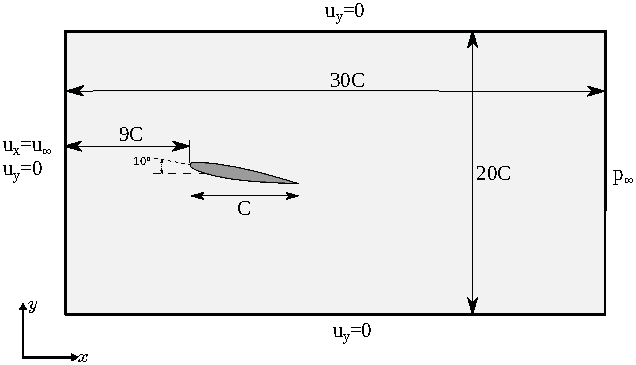
\includegraphics[scale=1.0,trim=0cm 0cm 0cm 0cm, clip=true]{Imagens/Cap6/aerofolio.pdf}}	
	\caption{Aerofólio 2D: Geometria}
	\label{fig:aerofolio2d_geometria}
\end{figure}

A análise é realizada para um número de Reynolds ($\Reynolds$) 1000 calculado a partir da dimensão do aerofólio e da velocidade de entrada do escoamento. Foram utilizados ainda como parâmetros de análise: $u_{\infty} = 1,0$,  $\rho = 1,0$,  $\timeStep = 0,02$, e $\specRadius = 0,75$.

Para validação da teoria apresentada nesse capítulo, compararam-se os resultados de coeficientes de arrasto e sustentação ao longo do tempo para duas discretizações distintas: 1. Monomodelo; 2. Combinação de duas malhas através do método Arlequin estabilizado.

O monomodelo foi discretizado através de elementos finitos (Fig. \ref{fig:aerofolio2d_malhamonomodelomef}), com malha constituída de 9240 elementos triangulares quadráticos e 18792 nós. 

\begin{figure}[htb!]
	\centering 
	{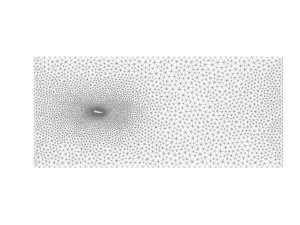
\includegraphics[scale=2.5,trim=0cm 0.9cm 0cm 0.8cm, clip=true]{Imagens/Cap6/malhaMonoEstatica.pdf}}	
	\caption{Aerofólio 2D: Malha Monomodelo (MEF) }
	\label{fig:aerofolio2d_malhamonomodelomef}
\end{figure}


Para o método Arlequin, duas malhas foram utilizadas, uma malha global em elementos isogeométricos (IGA) e uma malha local, mais refinada, em elementos finitos (MEF). Uma visão global da composição do domínio é apresentada na Fig. \ref{fig:aerofolio2d_dominioglobal}. Uma vista aproximada do aerofólio e da malha local pode ser visualizada na Fig. \ref{fig:aerofolio2d_dominiolocal}.

\begin{figure}[!htb]
	\centering
	\subfloat[Discretização da malha global (IGA) e local (MEF)\label{fig:aerofolio2d_dominioglobal}]{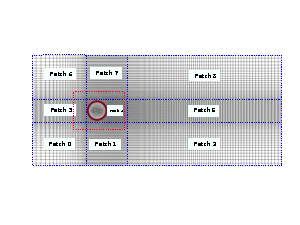
\includegraphics[scale=3.0,trim=0cm 1cm 0cm 0.6cm, clip=true]{Imagens/Cap6/malhaCoarseFinePatch.pdf}}\\
	\subfloat[Discretização próxima ao aerofólio \label{fig:aerofolio2d_dominiolocal}]{\includegraphics[trim=0 0 0 0,clip=true,scale=1.5]{Imagens/Cap6/DetalheFine.pdf}}
	\caption{Aerofólio 2D: Discretização das malhas}
	\label{fig:aerofolio2d_malhasepatches}
\end{figure}

A malha global em elementos isogeométricos quadráticos foi obtida através da utilização de 9 $patches$, que totalizaram 15561 pontos de controle. A malha local por sua vez é composta por 5214 elementos triangulares quadráticos e 10670 nós. 

Na Fig. \ref{fig:aerofolio2d_dominiolocal} pode observar em vermelho os elementos que fazem parte da zona de colagem. A espessura da zona de colagem foi definida como $0,2$, totalizando 628 elementos triangulares quadráticos e 1428 nós nessa região. A constante do operador de acoplamento $L^{2}$ foi definida como $k_{0} = 10$. 


Nesse problema observa-se o surgimento de uma esteira de vórtices a jusante do aerofólio, que resulta em um número de Strouhal ($\Strouhal$) equivalente a 0,877. Esse valor encontra-se em concordância com o obtido por \citeonline{MittalT:1994} de 0,862. 

Nas Fig. \ref{fig:aerofolio2d_aeroDrag} e Fig. \ref{fig:aerofolio2d_aeroLift} apresentam-se os resultados de coeficiente de arrasto e sustentação obtidos para as análises realizadas. Pode-se observar que os resultados obtidos com o modelo baseado no método Arlequin estabilizados estão de acordo com os obtidos para o modelo usando monomodelo.


\begin{figure}[htb!]
	\centering 
	{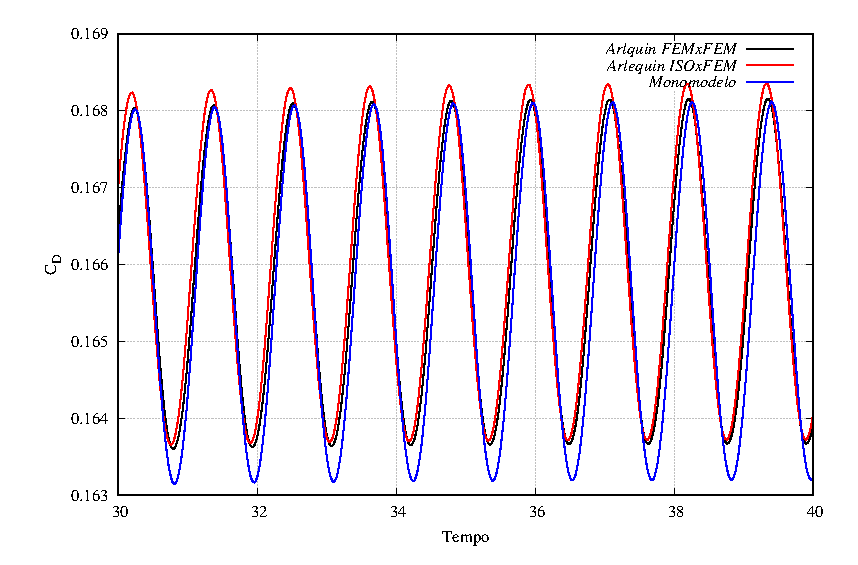
\includegraphics[scale=1.0,trim=0cm 0cm 0cm 0cm, clip=true]{Imagens/Cap6/DragRe.eps}}	
	\caption{Aerofólio 2D: Coeficiente de Arrasto}
	\label{fig:aerofolio2d_aeroDrag}
\end{figure}

\begin{figure}[htb!]
	\centering 
	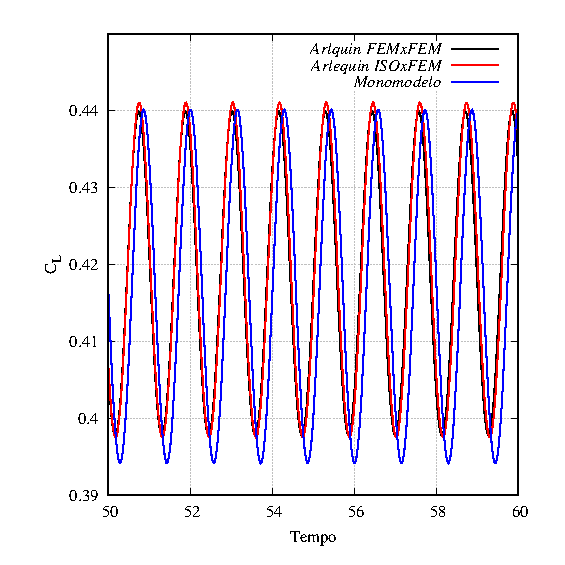
\includegraphics[scale=1.0,trim=0cm 0cm 0cm 0cm, clip=true]{Imagens/Cap6/LiftRe.eps}	
	\caption{Aerofólio 2D: Coeficiente de Sustentação}
	\label{fig:aerofolio2d_aeroLift}
\end{figure}

Nas Fig. \ref{fig:aerofolio2d_velocidadeestatica} e Fig. \ref{fig:aerofolio2d_pressaoestatica} estão apresentados os campos de velocidade e pressão respectivamente para um período de um ciclo das curvas referentes aos coeficientes de arrasto e sustentação. 

\begin{figure}[htb!]
	\centering
	\subfloat[$T_n$]{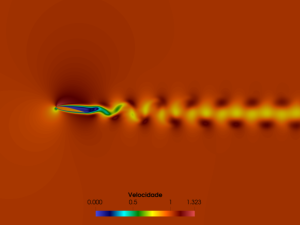
\includegraphics[scale=1.0,trim=0cm 0cm 0cm 0cm, clip=true]{Imagens/Cap6/velTn.pdf}} \ \
	\subfloat[$T_n + T_n/4$]{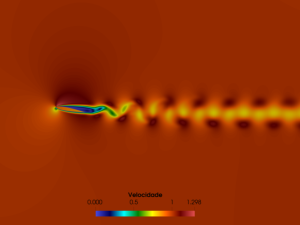
\includegraphics[trim=0 0 0 0,clip=true,scale=1.0]{Imagens/Cap6/velTn4.pdf}} \\
	\subfloat[$T_n + T_n/2 $]{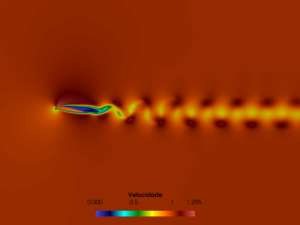
\includegraphics[scale=1.0,trim=0cm 0cm 0cm 0cm, clip=true]{Imagens/Cap6/velTn2.pdf}} \ \
	\subfloat[$T_n + 3T_n/4$]{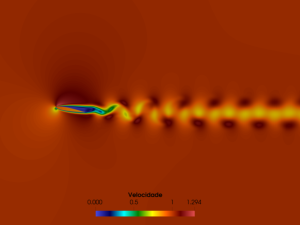
\includegraphics[trim=0 0 0 0,clip=true,scale=1.04]{Imagens/Cap6/velTn34.pdf}}
	\caption{Aerofólio 2D: Campo de velocidade}
	\label{fig:aerofolio2d_velocidadeestatica}
\end{figure}

\begin{figure}[htb!]
	\centering
	\subfloat[$T_n$]{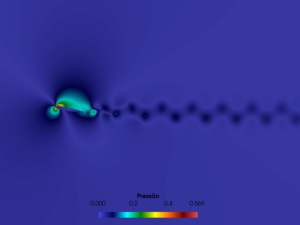
\includegraphics[scale=1.0,trim=0cm 0cm 0cm 0cm, clip=true]{Imagens/Cap6/pressTn.pdf}} \ \
	\subfloat[$T_n + T_n/4$]{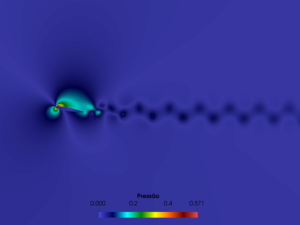
\includegraphics[trim=0 0 0 0,clip=true,scale=1.0]{Imagens/Cap6/pressTn4.pdf}} \\
	\subfloat[$T_n + T_n/2 $]{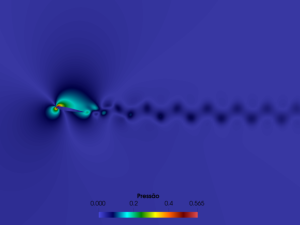
\includegraphics[scale=1.0,trim=0cm 0cm 0cm 0cm, clip=true]{Imagens/Cap6/pressTn2.pdf}} \ \
	\subfloat[$T_n + 3T_n/4$]{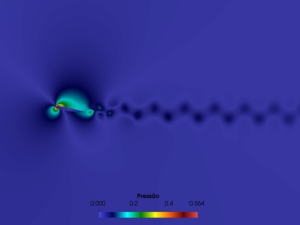
\includegraphics[trim=0 0 0 0,clip=true,scale=1.0]{Imagens/Cap6/pressTn34.pdf}}
	\caption{Aerofólio 2D: Campo de pressão}
	\label{fig:aerofolio2d_pressaoestatica}
\end{figure}


\subsection{Aerofólio com movimento de arfagem prescrito}


Para a validação computacional da técnica Arlequin estabilizada em domínios móveis  utilizou-se um problema envolvendo um aerofólio NACA 0012, semelhante ao apresentado na subseção anterior \ref{subsec:EX1NACA0012}, aplicando-se, entretanto, um movimento de arfagem ao mesmo. O aerofólio apresenta variação do ângulo de ataque em $20^{\circ}$, iniciando o movimento em $10^{\circ}$ e finalizando-o em $30^{\circ}$. 

Para descrever-se tal movimento aplica-se, tendo como centro a corda média do aerofólio, o movimento de rotação de corpo rígido através da seguinte relação:

\begin{align}
	\theta = \frac{\theta_{max}+\theta_{min}}{2} - \frac{\theta_{max}-\theta_{min}}{2}\cos{\omega_{f}t} ,
\end{align}

\noindent com $\omega_{f} = 2\pi f_{f}$, sendo $f_{f}$ a frequência de oscilação, adotada nesse estudo como 1.0, $\theta_{max} = 30^{\circ}$ e $\theta_{min} = 10^{\circ}$.

As dimensões da geometria do domínio computacional são alteradas (ver Fig. \ref{fig:AerofolioMoving}) para capturar os efeitos dos desprendimentos de vórtices, que para esse problema, se desprendem em uma faixa mais ampla. Os demais parâmetros de análise foram mantidos iguais aos apresentados no exemplo da subseção \ref{subsec:EX1NACA0012}. 

\begin{figure}[htb!]
	\centering 
	{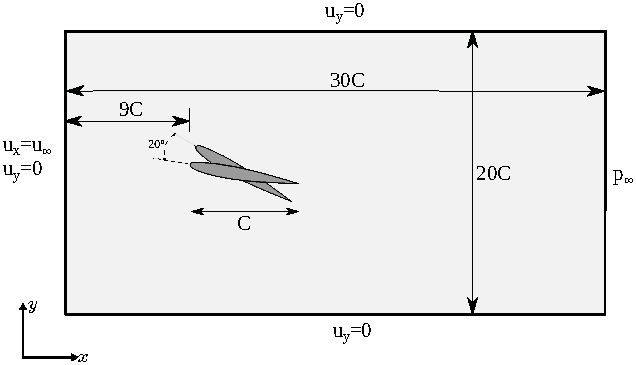
\includegraphics[scale=1.0,trim=0cm 0cm 0cm 0cm, clip=true]{Imagens/Cap6/aerofolioMov.pdf}}	
	\caption{Aerofólio Mov. 2D: Geometria}
	\label{fig:AerofolioMoving}
\end{figure}

Novamente são analisadas 2 discretizações: 1. Monomodelo; 2. Combinação de duas malhas através do método Arlequin estabilizado.
O monomodelo consiste em uma malha com 12438 elementos triangulares quadráticos e 25188 elementos. As malhas global e local do método Arlequin mantiveram-se com a mesma discretização do problema da subseção \ref{subsec:EX1NACA0012}, incluindo a quantidade de elementos na zona de colagem.

É importante ressaltar que para a simulação desse exemplo, utilizou-se como campo inicial de velocidade e pressão, valores obtidos em uma solução de longo termo do aerofólio na condição de repouso.

A variação dos coeficientes de arrasto e sustentação ao longo do tempo são apresentados nas Fig. \ref{fig:AeroDragMov} e Fig. \ref{fig:AeroLiftMov}. Nota-se nas imagens que o monomodelo e o modelo Arlequin estão consistentes em suas respostas. Soluções semelhantes podem ser observados no trabalho de \citeonline{Fernandes:2020}.

\begin{figure}[htb!]
	\centering 
	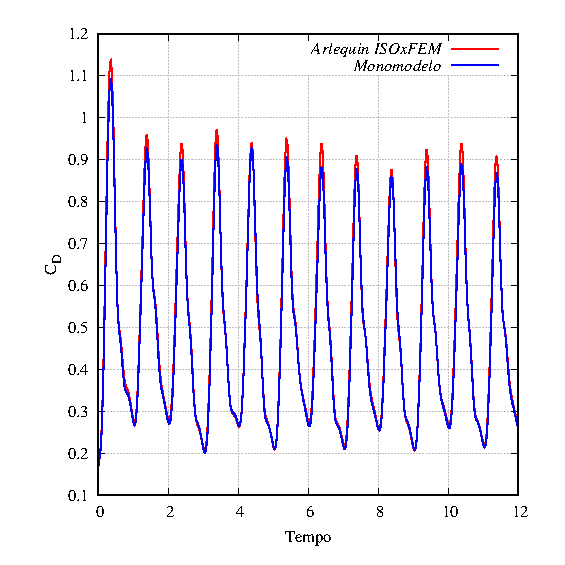
\includegraphics[scale=1.0,trim=0cm 0cm 0cm 0cm, clip=true]{Imagens/Cap6/DragMov.eps}	
	\caption{Aerofólio Mov. 2D: Coeficiente de Arrasto}
	\label{fig:AeroDragMov}
\end{figure}

\begin{figure}[htb!]
	\centering 
	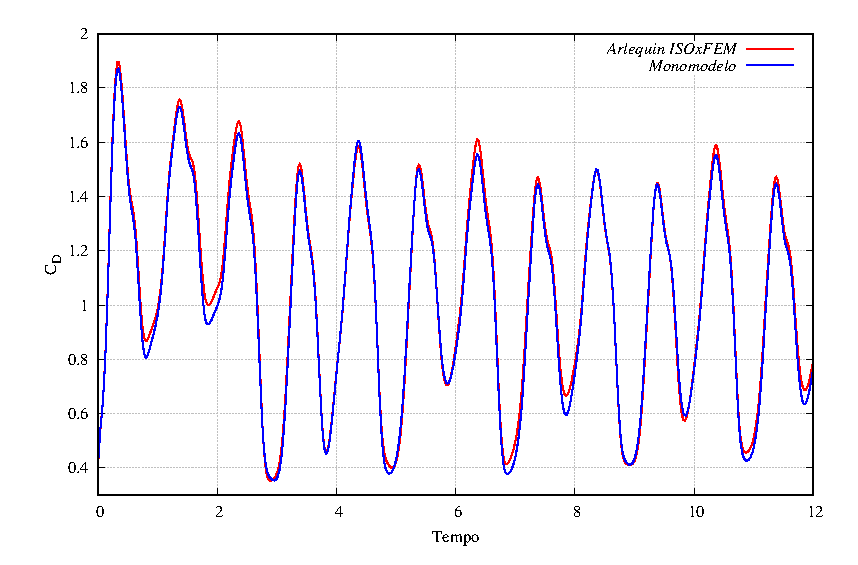
\includegraphics[scale=1.0,trim=0cm 0cm 0cm 0cm, clip=true]{Imagens/Cap6/LiftMov.eps}	
	\caption{Aerofólio Mov. 2D: Coeficiente de Sustentação}
	\label{fig:AeroLiftMov}
\end{figure}

Nas figuras Fig. \ref{fig:aerofolio2dMov_velocidade} e Fig. \ref{fig:aerofolio2dMov_pressao} são apresentados os campos de velocidade e pressão em alguns instantes para um ciclo do movimento oscilatório preescrito.

\begin{figure}[htb!]
	\centering
	\subfloat[$t = 8,0 $]{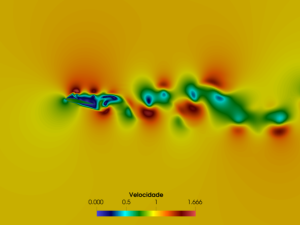
\includegraphics[scale=1.00,trim=0cm 0cm 0cm 0cm, clip=true]{Imagens/Cap6/vel400.pdf}} \
	\subfloat[$t = 8,3 $]{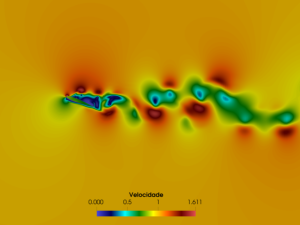
\includegraphics[trim=0 0 0 0,clip=true,scale=1.0]{Imagens/Cap6/vel413.pdf}}\\
	\subfloat[$t = 8,5 $]{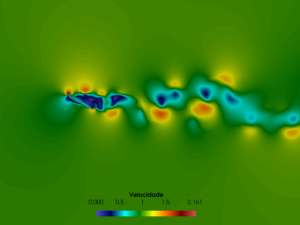
\includegraphics[scale=1.00,trim=0cm 0cm 0cm 0cm, clip=true]{Imagens/Cap6/vel425.pdf}} \
	\subfloat[$t = 8,8 $]{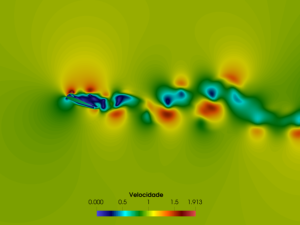
\includegraphics[trim=0 0 0 0,clip=true,scale=1.0]{Imagens/Cap6/vel438.pdf}}\\
	\subfloat[$t = 9,0 $]{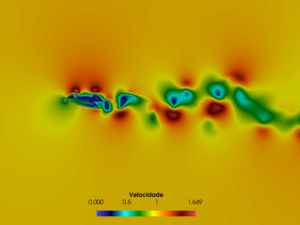
\includegraphics[trim=0 0 0 0,clip=true,scale=1.0]{Imagens/Cap6/vel450.pdf}}
	\caption{Aerofólio Mov. 2D: Campos de velocidade}
	\label{fig:aerofolio2dMov_velocidade}
\end{figure}

\begin{figure}[htb!]
	\centering
	\subfloat[$t = 8,0 $]{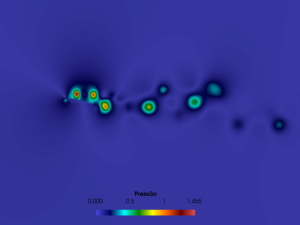
\includegraphics[scale=1.00,trim=0cm 0cm 0cm 0cm, clip=true]{Imagens/Cap6/press400.pdf}} \
	\subfloat[$t = 8,3 $]{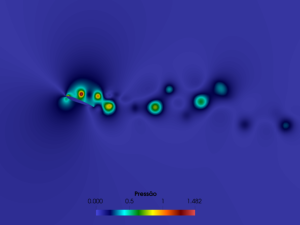
\includegraphics[trim=0 0 0 0,clip=true,scale=1.0]{Imagens/Cap6/press413.pdf}}\\
	\subfloat[$t = 8,5 $]{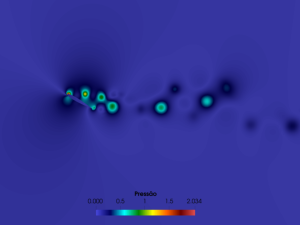
\includegraphics[scale=1.00,trim=0cm 0cm 0cm 0cm, clip=true]{Imagens/Cap6/press425.pdf}} \
	\subfloat[$t = 8,8 $]{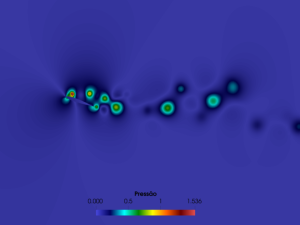
\includegraphics[trim=0 0 0 0,clip=true,scale=1.0]{Imagens/Cap6/press438.pdf}}\\
	\subfloat[$t = 9,0 $]{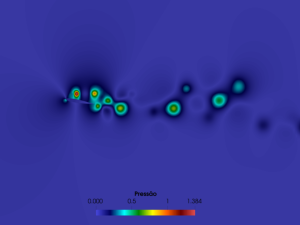
\includegraphics[trim=0 0 0 0,clip=true,scale=1.0]{Imagens/Cap6/press450.pdf}}
	\caption{Aerofólio Mov. 2D: Campos de pressão}
	\label{fig:aerofolio2dMov_pressao}
\end{figure}

\end{document}
